\newpage
\section{经典FOC的速度-电流双闭环PI控制实现}

经典的FOC速度-电流双闭环PI控制系统框图如下图所示。
\begin{figure}[H]
    \centering
    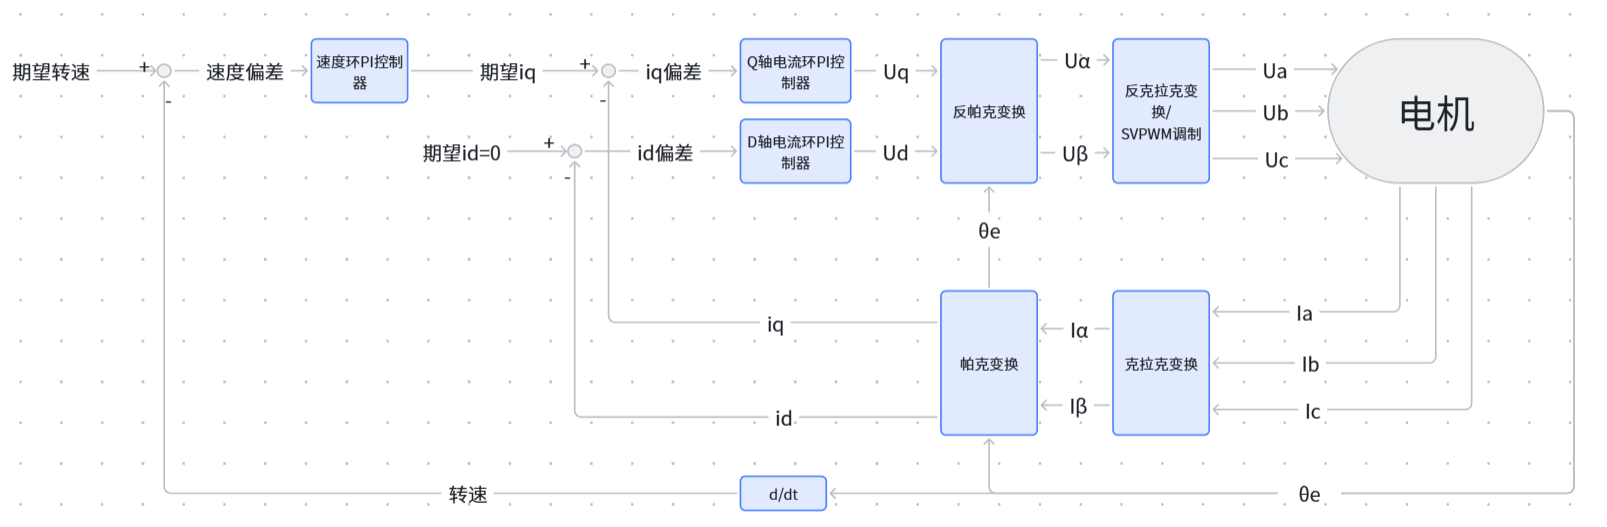
\includegraphics[width=0.8\textwidth]
    {图片/经典FOC控制结构框图.png}
    \caption{经典FOC控制结构框图}
    \label{fig:经典FOC控制结构框图}
\end{figure}
接下来将逐个介绍每个模块的实现。

\subsection{硬件设计}
一个完整的FOC控制系统硬件部分主要由以下几部分组成：主控MCU、电流传感器、转子位置传感器（编码器）、三相全桥驱动器、三相全桥电路、电源电路
、其他设备（如通信接口等）。

对于主控MCU，采用意法半导体的STMG431CBU6。其主频可达170MHz，并且支持DSP库，是意法半导体为电机驱动与控制而做了专门适配的微控制器。
开发过程中先使用核心板进行调试，相关电路如下图\ref{fig:核心板电路}所示。
\begin{figure}[H]
    \centering
    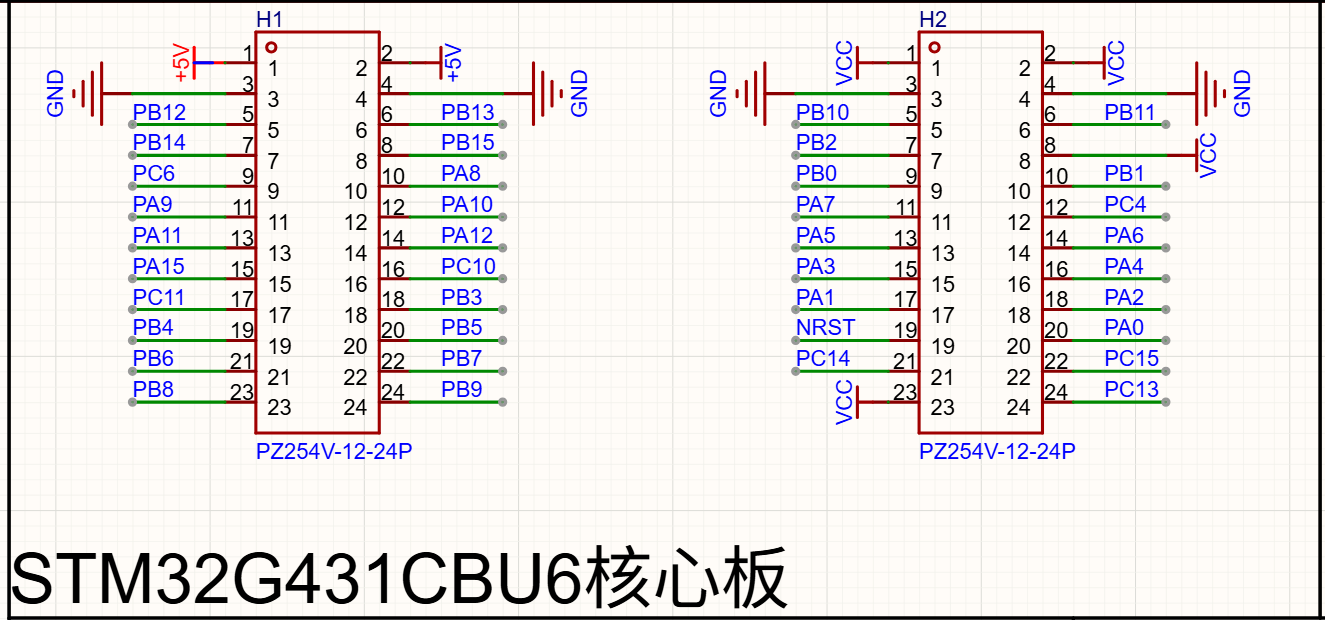
\includegraphics[width=0.5\textwidth]
    {图片/核心板电路.png}
    \caption{核心板电路}
    \label{fig:核心板电路}
\end{figure}

对于电流传感器，采用测流电阻+比例放大电路实现。为了节约电阻，选择两相低端检测的方案。即检测A，B两相的电流，C相电流通过基尔霍夫电流定律
通过$i_C=-i_A-i_B$来计算。考虑到被控设备为云台电机，标称额定电流不到1A，因此选择5mΩ作为电流检测电阻，比例放大电路放大系数配置为100。
此外，由于三相电路电流会出现负值，因此需要在比例放大电路中施加偏置。为了与MCU的ADC外设配合，选择偏置电压为ADC最大采集电压的一半，
即1.65V（通过电阻分压实现）。最终可得电流检测部分电路如下图\ref{fig:电流检测电路}所示，此时输出电压和单相电流之间的函数关系为：
\(U_o=1.65-0.5I\)
\begin{figure}[H]
    \centering
    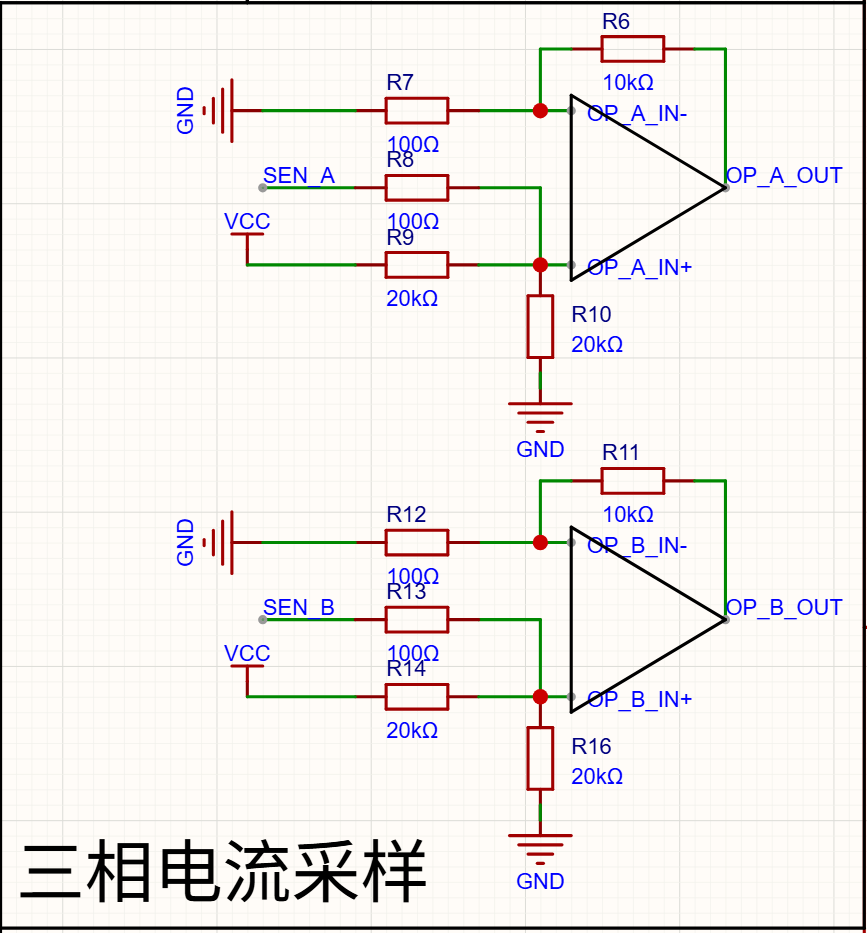
\includegraphics[width=0.5\textwidth]
    {图片/电流检测电路.png}
    \caption{电流检测电路}
    \label{fig:电流检测电路}
\end{figure}

转子位置传感器，也就是编码器，是区别于经典有感FOC和无感FOC的关键。此处选择为绝对式磁编码器，型号TLE5012BE1000。该型号传感为英飞凌公司
推出的高性能磁编码器，提供15位的绝对式角度检测分辨率，并且可以通过SSC通信协议（SPI兼容）实现与MCU的通信，驱动较为简单。为了给芯片提供
稳定的供电，选择将5V电压通过LDO降压到3.3V进行供电，通过LDO的高PSRR（电源抑制比）来确保编码器的稳定运行，并且也要通过LDO避免其他用电
电路对编码器的干扰。编码器相关电路如下图\ref{fig:编码器相关电路}所示。
\begin{figure}[H]
    \centering
    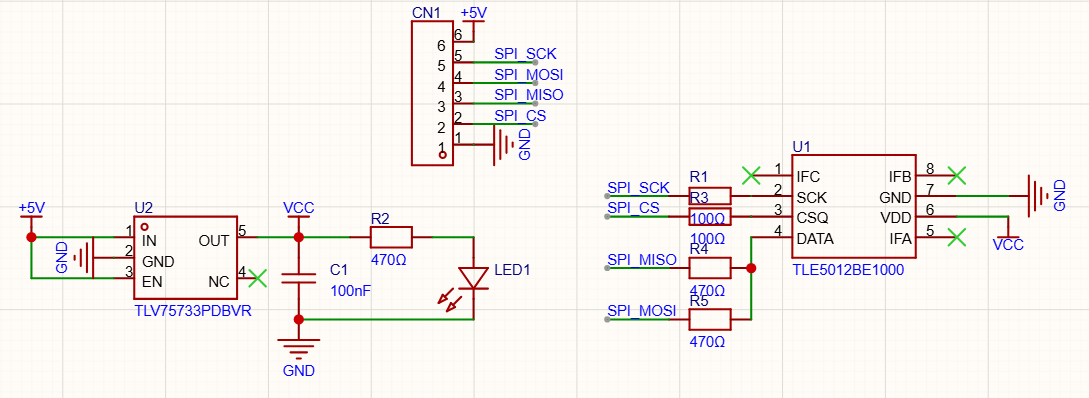
\includegraphics[width=0.5\textwidth]
    {图片/编码器相关电路.png}
    \caption{编码器相关电路}
    \label{fig:编码器相关电路}
\end{figure}

三相全桥驱动器和三相全桥电路是将PWM信号进行放大、直接实现对电机驱动的电路，其电路图与\ref{fig:三相全桥逆变电路}所示。
大部分方案选择将驱动器与电路本身分离，目的是通过用单独的功率器件构成三相全桥，提高带电机负载的能力。但是云台电机驱动电流小，
PCB设计空间有限，因此选择将驱动器与电路本身集成在一起，采用德州仪器的DRV8313作为一体式驱动器。DRV8313基于电荷泵原理实现对上桥的驱动
并且预留了每一相对应的接地端，便于通过测流电阻实现相电流检测。其单相瞬时最大电流可达2.5A，持续最大电流有效值可达1.75A，工作电压从8V到60V
，基本满足驱动云台电机的需要。相关电路图如下图\ref{fig:电机驱动电路}所示。
\begin{figure}[H]
    \centering
    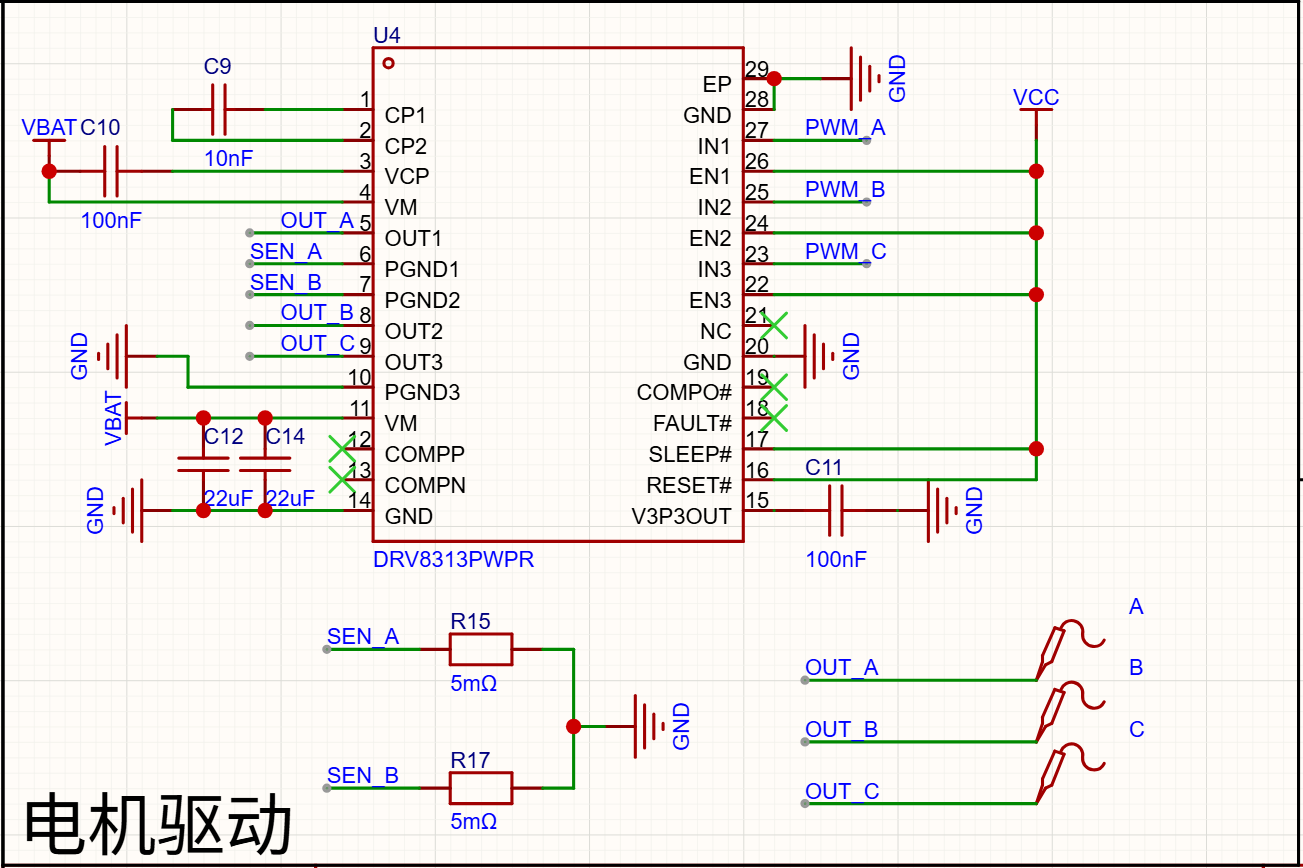
\includegraphics[width=0.5\textwidth]
    {图片/电机驱动电路.png}
    \caption{电机驱动电路}
    \label{fig:电机驱动电路}
\end{figure}

电源电路主要为各个电路提供各自需要的工作电压。对于主控MCU，需要3.3V工作电压；对于磁编码器，需要5V工作电压（之后再有编码器部分电路降压到
3.3V）；对于电机驱动电路，则是电池电压12V~24V。此外，为了确保安全，需要在电源输入端加入自恢复保险丝。
为了适应相关电压需求，采用典型的DC-DC大压差降压+LDO小压差降压方案，用DC-DC保证能量转换率，用LDO保证电压稳定性。

DC-DC采用德州仪器的LMR5140YYCR同步降压芯片，封装小（SOT-23-6）；开关频率高（1.1MHz），能够减小后续电感和电容的选型；最大输出电流2A，
足以满足控制逻辑电路供电需要；最大输入电压36V，能够匹配电机供电需要。

LDO采用德州仪器的TLV75733PDBVR，封装小（SOT-23-5），PSRR高（52dB@1MHz），能够提供稳定的3.3V电压。
电源电路相关电路如下图\ref{fig:电源电路}所示。
\begin{figure}[H]
    \centering
    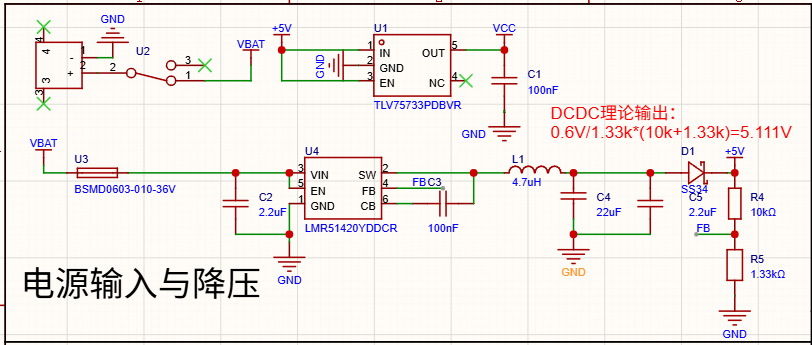
\includegraphics[width=0.5\textwidth]
    {图片/电源电路.png}
    \caption{电源电路}
    \label{fig:电源电路}
\end{figure}

其他设备包括电源指示灯、串口（向上位机发送数据）、母线电压采集电路（用于监控供电电压）等。值得一提的是母线电压检测电路。根据SVPWM计算公式
\eqref{eq:SVPWM占空比表达式}可以发现，计算三相占空比依赖母线电压$U_{dc}$。对于云台电机，工作电压范围为12V到24V，母线电压差距较大。为了
确保三相占空比计算正确，通过母线电压检测电路，让MCU通过ADC检测母线电压用于计算是很重要的。而供电一侧往往通过电池或可调直流电源实现，
电压波动较小，其主要信息集中在低频段，因此通过低通滤波电路滤除高频干扰，避免因为采集噪声导致三相占空比计算出错。
母线电压检测电路如下图\ref{fig:母线电压检测电路}所示。通过$R_4,R_5$实现$\cfrac{1.33k\Omega}{10k\Omega+1.33k\Omega}=0.1173$
的分压采集。在ADC最大输入电压3.3V情况下允许供电电压为$3.3V\div0.1173=28.13V$，足以覆盖电机供电电压。
通过$R_{7},C_6$构成RC低通滤波电路，上限截止频率为$\cfrac{1}{2\pi\times20k\Omega\times22uF}=0.36Hz$。
\begin{figure}[H]
    \centering
    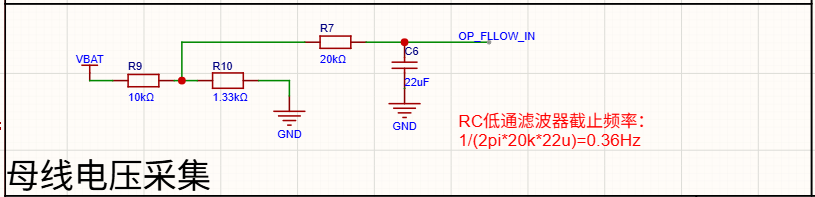
\includegraphics[width=0.5\textwidth]
    {图片/母线电压检测电路.png}
    \caption{母线电压检测电路}
    \label{fig:母线电压检测电路}
\end{figure}

\subsection{MCU外设配置与底层驱动程序}

MCU的外设配置主要关注ADC、TIM、SPI、UART等外设的配置，而底层驱动程序主要是磁编码器TLE5012B的驱动和上位机通信
撰写。两者同属底层驱动，因此在一节中讲述。使
用CLion+STM32CubeMX进行开发，因此外设配置主要在STM32CubeMX中进行图形化配置。

为了获取最高的程序运行速率，使能HSE和LSE，达到170MHz的主频。

为了实现电流检测电路中的比例放大，使能OPAMP1和OPAMP2两个模拟运算放大器外设，配置为独立模式，通过外部电阻网络构成带有直流偏置的比例放大电路。
然后将OPAMP1和OPAMP2外设的输出端连接到ADC外设，分别为ADC1$\_$IN3通道和ADC2$\_$IN3通道，将放大后的电压通过ADC采集实现电流检测。

为了实现母线电压检测，可以将母线电压检测电路的输出端连接到OPAMP3外设，并且将OPAMP3外设配置为跟随器模式，进一步提升输入阻抗，避免输入电流
带来的压降影响对母线电压的判断。同样地，将OPAMP3外设输出端连接到ADC外设，为ADC1$\_$IN12通道。

在电流环控制中，一般是每一个PWM周期都进行一次电流环控制。如果采用中断软件触发ADC采集会浪费很多时间，迫使PWM频率降低以适应计算需要的
长时间周期。因此较为简单的方法是采用硬件触发。针对ADC1和ADC2，使能注入组采集，触发源选择为TIM1的捕获比较事件4（Timer 1 Capture Compare
4 Event）。也就是说，每当TIM4$\_$CH4产生一次捕获比较事件后就会通过硬件直接触发注入组ADC采集，避免中断带来的软件延迟。

此外，由于ADC1$\_$IN3通道和ADC2$\_$IN3负责检测电机相电流，对于精度有较高的要求。而通过电阻分压得到的1.65V偏置电压会因为分压电阻
精度问题而略有偏差，需要在程序开始时进行零位矫正。通过使能规则组通道，采用软件触发即可。

接下来是核心外设定时器的配置。采用TIM1作为产生三相PWM的核心外设，预分频器PSC设置为0，计数模式选择为中心对齐模式3（Center Aligned Mode3）,
该模式下可以实现中心对齐PWM的产生。自动重装寄存器ARR设置为5664。此时PWM频率为
$f_{PWM}=\cfrac{170MHz}{2(0+1)(5664+1)}\approx 15.004kHz$，对应的电流环控制周期为66.647us。
使能TIM1$\_$CH1、TIM1$\_$CH2和TIM1$\_$CH3为PWM生成模式，用于产生三相PWM；
使能TIM1$\_$CH4为PWM生成无输出模式，将捕获比较寄存器CCR配置为ARR-1，用于产生捕获比较事件和捕获比较中断以开始电流环控制。

采用TIM2作为速度环控制中断的定时器，预分频器PSC设置为0，计数模式为向上计数，自动重装寄存器ARR设置为170000-1，此时更新中断频率为
$f_{INT}=\cfrac{170MHz}{(0+1)(170000-1+1)}= 1kHz$，对应的速度环控制周期为1ms。

通信接口在开发阶段主要使用SPI和UART。SPI通信用于和磁编码器TLE5012B进行通信，UART通信用于向上位机发送数据。根据TLE5012B数据手册，其采用
的SSC通信协议为MOSI和MISO合并为一条数据线的类SPI通信，因此将SPI外设配置为半双工主机模式（Half Duplex Master），选择软件片选；
为了尽可能减少与上位机通信占用的事件，将UART的波特率选择为2Mbps，采用奇校验，并使能DMA通道。

最后，由于FOC相关变换公式\eqref{eq:帕克变换}\eqref{eq:帕克逆变换}含有三角函数计算，采用\texttt{math.h}中的相关函数计算占用时间长，因此
一般选择查表+线性插值或硬件计算实现。STM32G431CBU6可以导入外部DSP库，也有CORDIC外设，两者都能大幅降低计算三角函数需要的事件。经过
测试发现，CORDIC外设计算三角函数时间略长于DSP库，因此采用DSP库实现三角函数计算。
\begin{figure}[H]
    \centering
    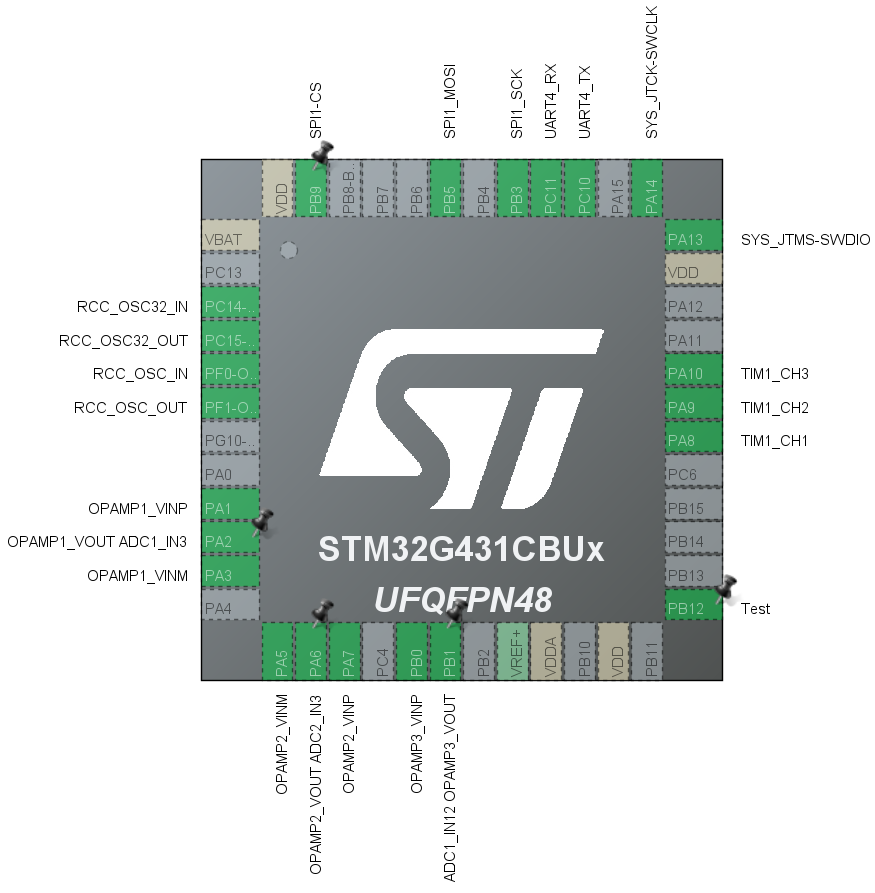
\includegraphics[width=0.5\textwidth]
    {图片/外设配置图.png}
    \caption{外设配置图}
    \label{fig:外设配置图}
\end{figure}

以上就是STM32G431CBU6的外设配置，结果如上图\ref{fig:外设配置图}所示。接下来进入底层驱动部分的撰写。

首先是对磁编码器TLE5012B的驱动文件撰写。定义头文件\texttt{MY$\_$TLE5012B.h}，包含指令码宏定义、片选信号产生与解除宏函数定义
和驱动函数声明：

\begin{lstlisting}
    #ifndef FOC_MY_TLE5012B_H
    #define FOC_MY_TLE5012B_H

    #include "main.h"

    //命令字
    #define CMD_READ_ANGLE_VALUE		0x8021  //读角度寄存器
    #define CMD_READ_SPEED_VALUE		0x8031  //读角速度寄存器
    #define CMD_READ_MOD2     0x8081  // 读配置寄存器 MOD2
    #define CMD_READ_MOD3     0x8091  // 读配置寄存器 MOD3
    #define CMD_WRITE_MOD2    0x0081  // 写配置寄存器 MOD2
    #define CMD_WRITE_MOD3    0x0091  // 写配置寄存器 MOD3

    //产生或取消片选信号宏函数定义
    #define SPI_CS_ENABLE HAL_GPIO_WritePin(SPI1_CS_GPIO_Port, SPI1_CS_Pin, GPIO_PIN_RESET);
    #define SPI_CS_DISABLE HAL_GPIO_WritePin(SPI1_CS_GPIO_Port, SPI1_CS_Pin, GPIO_PIN_SET);

    //读数据
    uint16_t TLE5012B_SPI_Read(uint16_t Order_Word);

    //写数据
    uint16_t TLE5012B_SPI_Write(uint16_t Order_Word, uint16_t WriteData);

    //读角度值
    double TLE5012B_Angle(void);

    //读角速度值
    double TLE5012B_Speed(void);

    #endif //FOC_MY_TLE5012B_H
\end{lstlisting}

定义源文件\texttt{MY$\_$TLE5012B.c}，主要是编写驱动程序的具体函数实现：

\begin{lstlisting}
    #include "MY_TLE5012B.h"

uint16_t TLE5012B_SPI_Read(uint16_t Order_Word) {
    uint16_t ReceiveData = 0;
    SPI_CS_ENABLE;
    HAL_SPI_Transmit(&hspi1, (uint8_t *) &Order_Word, 1,HAL_MAX_DELAY);
    HAL_SPI_Receive(&hspi1, (uint8_t *) &ReceiveData, 1,HAL_MAX_DELAY);
    ReceiveData = ReceiveData & 0x7FFF; //舍弃最高位状态位
    SPI_CS_DISABLE;
    return ReceiveData;
}

uint16_t TLE5012B_SPI_Write(uint16_t Order_Word, uint16_t WriteData) {
    SPI_CS_ENABLE;
    uint16_t Data[2] = {Order_Word, WriteData};
    HAL_SPI_Transmit(&hspi1, (uint8_t *) Data, 2, HAL_MAX_DELAY);
    HAL_Delay(1);
    SPI_CS_DISABLE;
    HAL_Delay(10);
}

double TLE5012B_Angle(void) {
    uint16_t Data = TLE5012B_SPI_Read(CMD_READ_ANGLE_VALUE);
    double Angle = Data * 360.0 / 32768;
    return Angle;
}

double TLE5012B_Speed(void) {
    uint16_t raw_data = TLE5012B_SPI_Read(CMD_READ_SPEED_VALUE);
    int16_t speed_counts = 0;
    if (raw_data & 0x4000) {
        //符号位为1，负数
        speed_counts = (int16_t) (raw_data | 0x8000);
    } else {
        //符号位为0，正数
        speed_counts = (int16_t) raw_data;
    }

    float delta_angle = (speed_counts / 32768.0) * 360.0;
    float omega_rad_s = delta_angle / 42.7e-6;
    return (double)omega_rad_s;
}

\end{lstlisting}

在函数\texttt{uint16$\_$t TLE5012B$\_$SPI$\_$Read(uint16$\_$t Order$\_$Word)}中，采用阻塞式SPI发送和接收函数，主要是因为在
半双工模式下需要手动切换目前SPI的状态是发送还是接收，不便于使用DMA。此外\texttt{double TLE5012B$\_$Speed(void)}函数
仅作为驱动测试，实际控制中由于读取一次数据花费时间较长，对于速度的计算一般通过角度之差实现。

另外需要编写与上位机通信相关的函数。为了减少通信占用的事件，加快通信频率，选择每一次速度环控制周期进行一次数据上传。
通信协议采用JUSTFLOAT协议，只传递\texttt{float}类型的数据。定义头文件\texttt{MY$\_$JUSTFLOAT.h}和源文件\texttt{MY$\_$JUSTFLOAT.c}
如下所示。

\begin{lstlisting}
    #ifndef FOC_MY_JUSTFLOAT_H
    #define FOC_MY_JUSTFLOAT_H

    #include "main.h"

    //JustFloat协议帧尾
    #define JUSTFLOAT_FRAME_TAIL 0x7F800000u
    //最大变量数
    #define JUSTFLOAT_MAX_VAR 16

    //串口句柄指针
    static UART_HandleTypeDef *jf_huart = NULL;

    //变量列表和变量数
    static float *jf_var_list[JUSTFLOAT_MAX_VAR];
    static uint8_t jf_var_cnt = 0;

    //实际发送数据：变量+帧尾
    static uint32_t jf_tx_buf[JUSTFLOAT_MAX_VAR + 1];

    //初始化JustFloat函数
    void JUSTFLOAT_Init(void);

    //绑定串口
    void JUSTFLOAT_BindUart(UART_HandleTypeDef *huart);

    //添加新变量
    void JUSTFLOAT_AddData(float *Data);

    //发送变量列表
    void JUSTFLOAT_SendData(void);

    #endif
\end{lstlisting}

\begin{lstlisting}
    #include "MY_JUSTFLOAT.h"

    void JUSTFLOAT_Init(void) {
        jf_var_cnt = 0;
        for (int i=0;i<JUSTFLOAT_MAX_VAR;i++) {
            jf_var_list[i] = NULL;
        }
    }

    void JUSTFLOAT_BindUart(UART_HandleTypeDef *huart) {
        jf_huart = huart;
    }

    void JUSTFLOAT_AddData(float *Data) {
        if (jf_var_cnt < JUSTFLOAT_MAX_VAR){
            jf_var_list[jf_var_cnt] = Data;
        }
        jf_var_cnt++;
    }

    void JUSTFLOAT_SendData(void) {
        uint8_t i;
        for (i = 0; i < jf_var_cnt; i++)
        {
            jf_tx_buf[i] = *(uint32_t *)jf_var_list[i];
        }
        jf_tx_buf[jf_var_cnt] = JUSTFLOAT_FRAME_TAIL;
        HAL_UART_Transmit_DMA(jf_huart,(uint8_t *)jf_tx_buf,(jf_var_cnt + 1) * sizeof(uint32_t));
    }
\end{lstlisting}

\subsection{程序初始化}

程序初始化过程是指从上电开始到进入主控制中断的过程，主要包括变量声明、外设启动、传感器零位标定三个步骤。

声明全局变量如下：

\begin{lstlisting}
//ADC采样原始数据
uint32_t ADC_Data[3] = {0, 0, 0};
//ADC采样转换后电流数据
float Current_abc[3] = {0, 0, 0};
//机械角度
float theta_m = 0;
float theta_m_last = 0;
//电角度
float theta_e = 0;
float Sin_theta_e = 0;
float Cos_theta_e = 0;
//机械角速度
float n_m = 0;
//速度环低通滤波
float n_m_last = 0;
//零位偏置
float ADC1_ZERO = 0;
float ADC2_ZERO = 0;
float Angel_ZERO = 0;
//两相静止坐标系电流
float I_alpha = 0;
float I_beta = 0;
//同步旋转坐标系电流
float I_d = 0;
float I_q = 0;
//SVPWM得到的三相占空比
float Duty_A = 0;
float Duty_B = 0;
float Duty_C = 0;
//母线电压
float Udc = U_DC_Default;
//SVPWM最大电压
float U_svpwm_max = U_DC_Default / SQRT3;
//DQ轴驱动电压
float U_d = 0;
float U_q = 0;
//电流-速度环PID控制器
Discrete_PID_Struct D_PID, Q_PID, Speed_PID;
//指令接收全局变量
uint8_t UART_Buffer[100];
float Order = 0;
uint16_t UART_Length = 0;
//电流环运行标志位
bool Current_Control_Flag = false;
\end{lstlisting}

并且宏定义可调参数如下：

\begin{lstlisting}
//数学常数
#define SQRT3 1.7320508065

//电机极对数
#define MOTOR_POLE_PAIRS 14

//速度环一阶低通滤波系数
#define Speed_Filter 0.1

//D轴电流环连续域PID参数
#define D_Kp 30
#define D_Ki 10000
#define D_Kd 0
#define D_N 10000

//Q轴电流环连续域PID参数
#define Q_Kp 30
#define Q_Ki 10000
#define Q_Kd 0
#define Q_N 10000

//速度环连续域PID参数
#define Speed_Kp 0.001
#define Speed_Ki 0.005
#define Speed_Kd 0
#define Speed_N 100

//速度环和电流环采样周期，单位s
#define Ts_Current ((__HAL_TIM_GET_AUTORELOAD(&htim1)+1)/170000000.0) * 2
#define Ts_Speed    ((__HAL_TIM_GET_AUTORELOAD(&htim2)+1)/170000000.0)

//默认母线电压，单位V
#define U_DC_Default 12

//默认给定电流，单位A
#define ID_Target_Default 0
#define IQ_Target_Default 0
//默认给定转速，单位rpm
#define Speed_Target_Default 0

//速度环输出限幅（电流环给定限幅）
#define Speed_Output_Limit 0.5

//速度环给定限幅
#define Speed_Target_Limit 350
\end{lstlisting}

完成变量声明后进行外设启动和传感器校准，两者一般分模块同时进行。

首先使能模拟运算放大器OPAMP1、OPAMP2和OPAMP3、使能ADC1和ADC2的规则组。此时TIM1和TIM2没有使能，不输出PWM，因此此时三相电流
均为零，直接采集OPAMP1和OPAMP2的输出电压，应该就是空载时的直流偏置电压。通过ADC1和ADC2的规则组阻塞式采样10次取均值，即可实现
直流偏置电压的采集。最后使能ADC1和ADC2的注入组并开启中断。代码段如下所示。

\begin{lstlisting}
    //使能模拟运算放大器
    HAL_OPAMP_Start(&hopamp1);
    HAL_OPAMP_Start(&hopamp2);
    HAL_OPAMP_Start(&hopamp3);

    //开启两个ADC校验
    HAL_ADCEx_Calibration_Start(&hadc1, ADC_SINGLE_ENDED);
    HAL_ADCEx_Calibration_Start(&hadc2, ADC_SINGLE_ENDED);
    for (int i = 0; i < 10; i++) {
        //ADC零位检测
        HAL_ADCEx_Calibration_Start(&hadc1, ADC_SINGLE_ENDED);
        HAL_ADCEx_Calibration_Start(&hadc2, ADC_SINGLE_ENDED);
        HAL_ADC_Start(&hadc1);
        if (HAL_ADC_PollForConversion(&hadc1, HAL_MAX_DELAY) == HAL_OK) {
            ADC1_ZERO += HAL_ADC_GetValue(&hadc1) / 4096.0 * 3.3;
        }
        HAL_ADC_Start(&hadc2);
        if (HAL_ADC_PollForConversion(&hadc2, HAL_MAX_DELAY) == HAL_OK) {
            ADC2_ZERO += HAL_ADC_GetValue(&hadc2) / 4096.0 * 3.3;
        }
    }
    ADC1_ZERO = ADC1_ZERO / 10.0;
    ADC2_ZERO = ADC2_ZERO / 10.0;
    //使能ADC注入组转换
    HAL_ADCEx_InjectedStart_IT(&hadc1);
    HAL_ADCEx_InjectedStart_IT(&hadc2);
\end{lstlisting}

然后进行编码器零位校准。这一部分主要是为了校准通过磁编码器读取计算出来的电角度。
考虑实际同步旋转坐标系如下图\ref{fig:控制坐标系和实际坐标系}
黑色部分所示，紫色部分是控制器所在的坐标系（控制坐标系），两者存在电角度偏差$\Delta \theta$满足
$\theta_{real}=\theta_{control}+\Delta\theta$
。设$U_d,U_q$表示实际坐标系的驱动电压，
而$U_{d_c},U_{q_c}$表示控制坐标系下的驱动电压。
\begin{figure}[H]
    \centering
    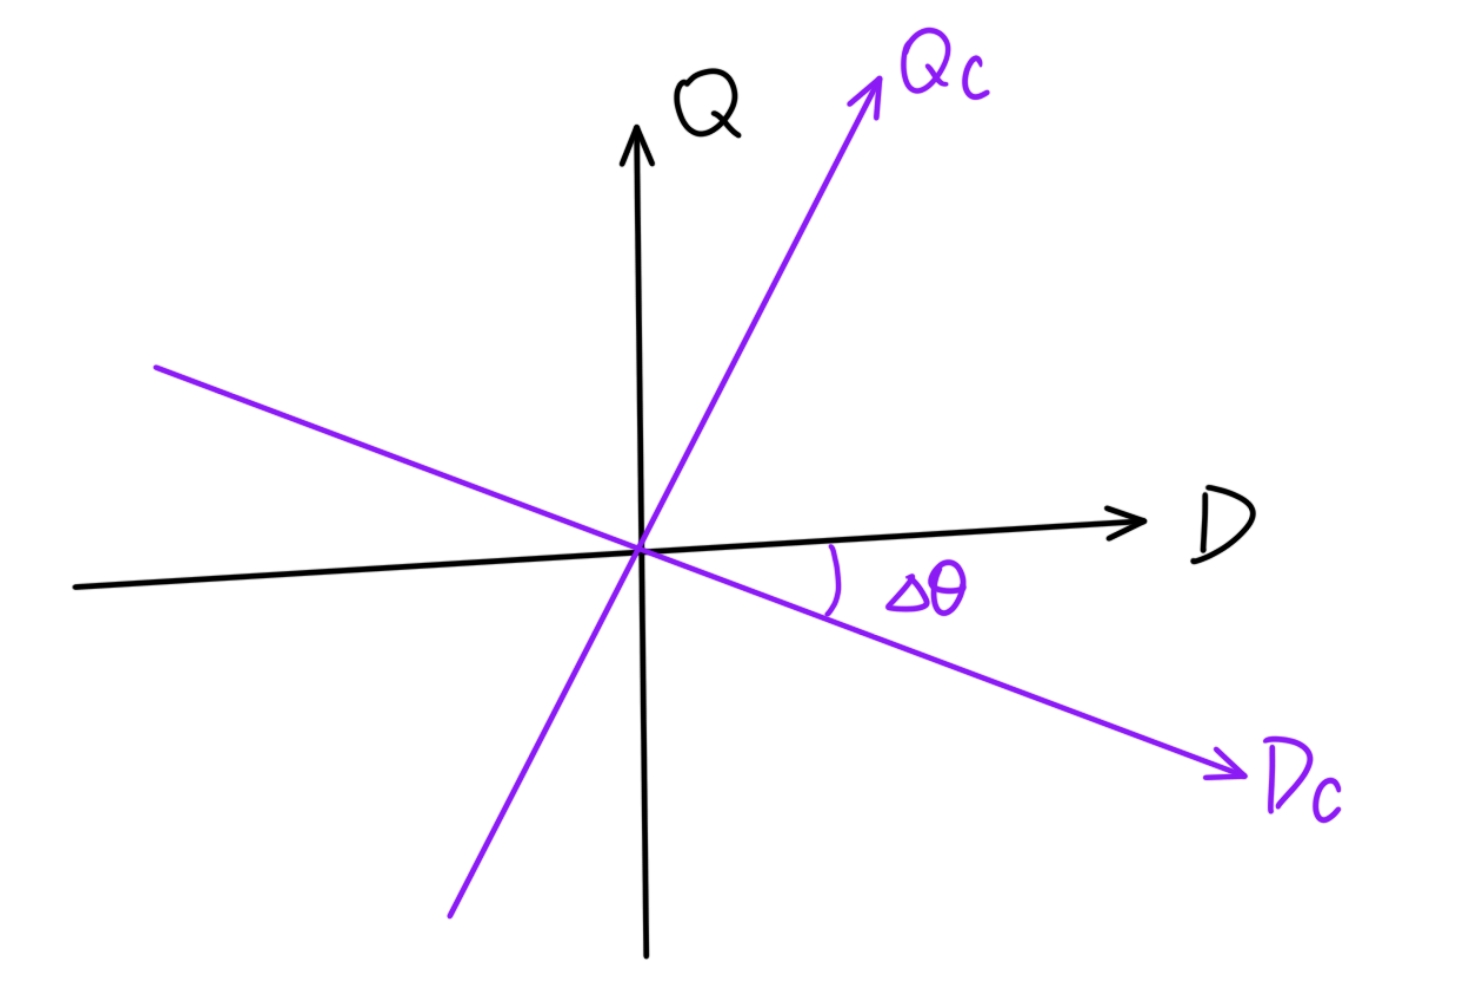
\includegraphics[width=0.3\textwidth]
    {图片/控制坐标系和实际坐标系.jpg}
    \caption{控制坐标系和实际坐标系}
    \label{fig:控制坐标系和实际坐标系}
\end{figure}

根据电磁转矩表达式\eqref{eq:同步坐标系下电磁转矩表达式（一般形式）}，可以发现$T_e\propto i_q$。而根据电路方程
\eqref{eq:同步坐标系下电路方程}可知，在初始无角速度情况下，只有通过给定$U_q$，才能使电机产生电磁转矩，使得电机旋转。
若只给定$U_d$，则电机不会旋转。根据图\ref{fig:控制坐标系和实际坐标系}可知，在给定$U_{d_c}$的情况下，编码器零位校准正确
的判别方法就是电机不发生旋转。
因此最简单的方法就是从零开始，按照特定步长递增，尝试每一个可能的$\Delta\theta$，直到电机在给定$U_d$持续一定时间
后角度增量小到可接受程度。这种方法需要长时间校准。为了解决这个问题，可以采用粗校准+细校准两部分来进行。

粗校准主要目的是缩小偏差的范围。
将编码器零位的可取范围用单位圆表示，特殊角0°、90°、180°、270°将其分为四个象限。以第一象限为例推导粗校准过程，如下图所示。
\begin{figure}[H]
    \centering
    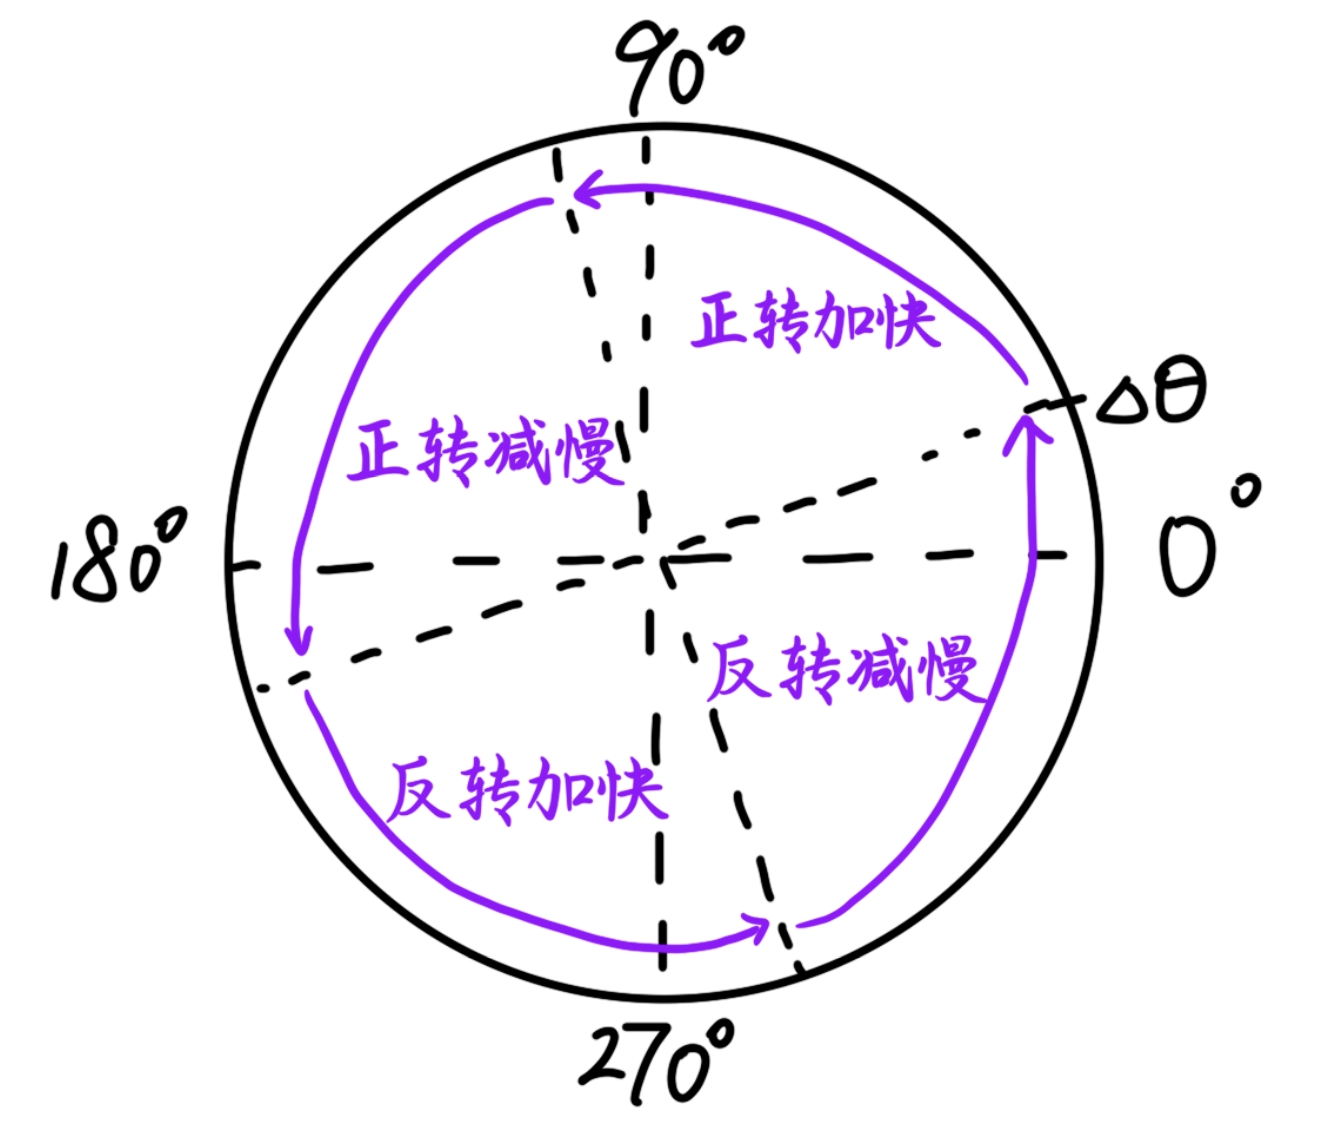
\includegraphics[width=0.3\textwidth]
    {图片/粗校准过程.jpg}
    \caption{粗校准过程}
    \label{fig:粗校准过程}
\end{figure}

假设当$U_q>0$时产生的电磁转矩在空载情况下使电机旋转的方向为正向。那么从0°开始不断增大尝试的电角度偏差，会经历反转减慢、正转加快、正转减慢
反转加快四个步骤。由于$\Delta\theta$位于第一象限，因此在0°和90°下测试得到的转速方向是不一致的（异号）。而在90°下测试得到的转速是正转的。
不难想到，通过判断0°和90°转速方向是否一致，可以判断$\Delta\theta$位于第一、第三象限还是位于第二、第四象限。而判断90°下测试得到的转速方向
就可以进一步确定$\Delta\theta$的象限，也就确定了基准值。
值得注意的是，0°和90°测试不具有唯一性，理论上只要是两个相差90°的特殊角都可以。最终得到象限判断表如下表\ref{tab:粗校准表}所示。
\begin{table}[H]
    \centering
    \begin{tabular}{|c|c|c|}
        \hline
        &90°测试点正转&90°测试点反转\\
        \hline
        90°和0°测试点转速方向相异&第一象限（0°基准）&第三象限（180°基准）\\
        \hline
        90°和0°测试点转速方向相同&第四象限（270°基准）&第二象限（90°基准）\\
        \hline
    \end{tabular}
    \caption{粗校准表}
    \label{tab:粗校准表}
\end{table}

接下来进行细校准过程。可以在粗校准基准值基础上通过特定步长自增来不断尝试$\Delta\theta$，但这同样需要较长时间。
可以从另一个角度分析，不妨假设这一过程为闭环控制：期望角速度为0，根据反馈得到的角速度偏差（$-\omega_m$），
执行特定控制律输出尝试的编码器零位，直到给定$U_d$运行一段时间电机角度基本不发生变化。

为了方便起见，假设控制器为I控制器，即下一步尝试的编码器零位满足$\Delta\theta_{next}=\Delta\theta_{current}-K_i\omega_m$。
加上校准步骤前使能TIM1和三相PWM，校准后使能电流环和速度环控制中断通道，最终得到的编码器零位校准程序如下所示。

\begin{lstlisting}
    //使能定时器
    HAL_TIM_Base_Start(&htim1);
    //三相PWM输出
    HAL_TIM_PWM_Start(&htim1, TIM_CHANNEL_1);
    HAL_TIM_PWM_Start(&htim1, TIM_CHANNEL_2);
    HAL_TIM_PWM_Start(&htim1, TIM_CHANNEL_3);
    //编码器零位校准
    int k = 0;
    Ud = 12;
    Uq = 0;
    // 基于I闭环控制模型抽象的编码器零位矫正
    int k = 0;
    U_d = U_svpwm_max;
    U_q = 0;
    float wm_0_90[2] = {0};
    for (int i = 0; i < 2; i++)
    {
      //读取起始机械角度
      theta_m_last = TLE5012B_Angle();
      // 给定Ud情况下转动
      for (int j = 0; j < 50; j++)
      {
        theta_e = TLE5012B_Angle();
        theta_e = theta_e * MOTOR_POLE_PAIRS + i * 90;
        DSP_Float_Calc_SinCos(theta_e, &Sin_theta_e, &Cos_theta_e);
        SVPWM_Calculation(&U_d, &U_q, Sin_theta_e, Cos_theta_e,U_svpwm_max, Udc, 
          &Duty_A, &Duty_B, &Duty_C);
        Set_CCR(Duty_A, Duty_B, Duty_C);
      }
      // 读取结束机械角度
      theta_m = TLE5012B_Angle();
      wm_0_90[i] = theta_m - theta_m_last;
      U_d = U_svpwm_max;
    }
    if (wm_0_90[0] * wm_0_90[1] < 0)
    {
      //零位位于第一、第三象限
      if (wm_0_90[1] < 0)
      {
        //零位位于第三象限
        Angel_ZERO = 180;
      }
      else if (wm_0_90[1] > 0)
      {
        //零位位于第一象限
        Angel_ZERO = 0;
      }
    }
    else if (wm_0_90[0] * wm_0_90[1] > 0)
    {
      //零位位于第二、第四象限
      if (wm_0_90[1] < 0)
      {
        //零位位于第二象限
        Angel_ZERO = 90;
      }
      else if (wm_0_90[1] > 0)
      {
        //零位位于第四象限
        Angel_ZERO = 270;
      }
    }
    while (k < 3)
    {
      float Angle_ZERO_Init = Angel_ZERO;
      theta_m_last = TLE5012B_Angle();
      for (int i = 0; i < 100; i++)
      {
        theta_e = TLE5012B_Angle();
        theta_e = theta_e * MOTOR_POLE_PAIRS + Angel_ZERO;
        DSP_Float_Calc_SinCos(theta_e, &Sin_theta_e, &Cos_theta_e);
        SVPWM_Calculation(&U_d, &U_q, Sin_theta_e, Cos_theta_e,U_svpwm_max, Udc, 
          &Duty_A, &Duty_B, &Duty_C);
        Set_CCR(Duty_A, Duty_B, Duty_C);
      }
      theta_m = TLE5012B_Angle();
      n_m = (1 - Speed_Filter) * (theta_m - theta_m_last) + Speed_Filter * n_m;
      U_d = U_svpwm_max;
      if (n_m < 0.5 && n_m > -0.5)
      {
        k++;
      }
      else
      {
        k = 0;
        Angel_ZERO += 0.1 * n_m;
      }
    }
\end{lstlisting}

经过测试，在选取合适的参数情况下，上述编码器零位校准方法能够较快的完成校准，但是重复性较差，且I控制参数和阈值选取不正确会导致
电机长时间卡死在校准中，无法正常进入工作状态。
此外该方法本质仍是试验方法，只不过使用I控制器的抽象和粗校准+细校准的分段方式加快的试验确定零位的速度。

另一种工业上常用的校准方法为定点测量。在A-B-C三相自然坐标系中，若给定A相电压，BC相电压很小，则磁链会被吸引到与A方向重合，此时应为
电角度的0°。为了避免单次校准误差，可以轮流给定A-B-C相电压，对应的理论电角度为0°、120°和240°。通过多次测量取平均，可以快速实现对
编码器零位的校准。校准程序如下。
\begin{lstlisting}
    int k = 0;
    U_d = U_svpwm_max;
    while(k<10)
    {
      //A相
      Set_CCR(0.9,0.1,0.1);
      HAL_Delay(500);
      theta_e = TLE5012B_Angle() * MOTOR_POLE_PAIRS;
      theta_e = fmod(theta_e, 360);
      theta_e<0?theta_e+=360:theta_e;
      Angel_ZERO += 360 - theta_e;
      //B相
      Set_CCR(0.1,0.9,0.1);
      HAL_Delay(500);
      theta_e = TLE5012B_Angle() * MOTOR_POLE_PAIRS - 120;
      theta_e = fmod(theta_e, 360);
      theta_e<0?theta_e+=360:theta_e;
      Angel_ZERO += 360 - theta_e;  
      //C相
      Set_CCR(0.1,0.1,0.9);
      HAL_Delay(500);
      theta_e = TLE5012B_Angle() * MOTOR_POLE_PAIRS + 120;
      theta_e = fmod(theta_e, 360);
      theta_e<0?theta_e+=360:theta_e;
      Angel_ZERO += 360 - theta_e;
      //计算零位
      Angel_ZERO = Angel_ZERO / 3;
      //验证
      theta_m_last = TLE5012B_Angle();
      for (int i = 0; i < 100; i++)
      {
        theta_e = TLE5012B_Angle();
        theta_e = theta_e * MOTOR_POLE_PAIRS + Angel_ZERO;
        DSP_Float_Calc_SinCos(theta_e, &Sin_theta_e, &Cos_theta_e);
        SVPWM_Calculation(&U_d, &U_q, Sin_theta_e, Cos_theta_e, U_svpwm_max, Udc, &Duty_A, &Duty_B, &Duty_C);
        Set_CCR(Duty_A, Duty_B, Duty_C);
      }
      theta_m = TLE5012B_Angle();
      n_m = (1 - Speed_Filter) * (theta_m - theta_m_last) + Speed_Filter * n_m;
      U_d = 0;
      if (n_m < 0.5 && n_m > -0.5)
      {
        break; 
      }
      else {
        k++;
        Angel_ZERO = 0;
      }
    }
\end{lstlisting}

最后一步为JUSTFLOAT相关通信协议注册变量并绑定串口，程序如下所示。

\begin{lstlisting}
    //初始化
    JUSTFLOAT_Init();
    //绑定串口
    JUSTFLOAT_BindUart(&huart4);
    //注册变量表
    JUSTFLOAT_AddData(&theta_m);
    JUSTFLOAT_AddData(&theta_e);
    JUSTFLOAT_AddData(&n_m);
    JUSTFLOAT_AddData(&Udc);
    JUSTFLOAT_AddData(&I_d);
    JUSTFLOAT_AddData(&I_q);
    // JUSTFLOAT_AddData(&Duty_A);
    // JUSTFLOAT_AddData(&Duty_B);
    // JUSTFLOAT_AddData(&Duty_C);
    JUSTFLOAT_AddData(&Angel_ZERO);
    JUSTFLOAT_AddData(&U_d);
    JUSTFLOAT_AddData(&U_q);
    JUSTFLOAT_AddData(&D_PID.Setvalue);
    JUSTFLOAT_AddData(&Q_PID.Setvalue);
    JUSTFLOAT_AddData(&Speed_PID.Setvalue);
    JUSTFLOAT_AddData(&Current_abc[0]);
    JUSTFLOAT_AddData(&Current_abc[1]);
    JUSTFLOAT_AddData(&Current_abc[2]);
\end{lstlisting}

\subsection{电流内环PI闭环控制}

电流内环PI控制由TIM1$\_$CH4的比较捕获事件/中断触发，主要包含数据采集、克拉克-帕克变换求取$I_d,I_q$、DQ轴PID控制运算、SVPWM调制、设定
三相占空比几个步骤。

数据采集包括对转子位置的采集和对三相电流的采集。由于三相电流采集通过比较捕获事件触发，触发速度远超中断，因此选择在比较捕获中断中通过与
磁编码器TLE5012B的通信获取转子位置。而由于通信需要的时间较长，因此在比较捕获中断过程中会被ADC注入组转换完成中断打断。但是由于ADC1和ADC2都
会采集数据、都会触发注入组转换完成中断。为了避免重复计算，考虑到ADC1需要对两个通道（一个A相电流，一个母线电压）转换而ADC2只需要对
一个通道转换，即ADC1总是比ADC2慢转换完成，因此可以只在ADC1转换完成后进行数据处理（还原电流、进行电流低通滤波、计算C相电流）。
又由于ADC注入组转换完成中断优先级较高，会比比较捕获中断更先执行完，因此将后续控制函数入口放在比较捕获中断末尾。数据采集流程图和程序段
如下所示。
\begin{figure}[H]
    \centering
    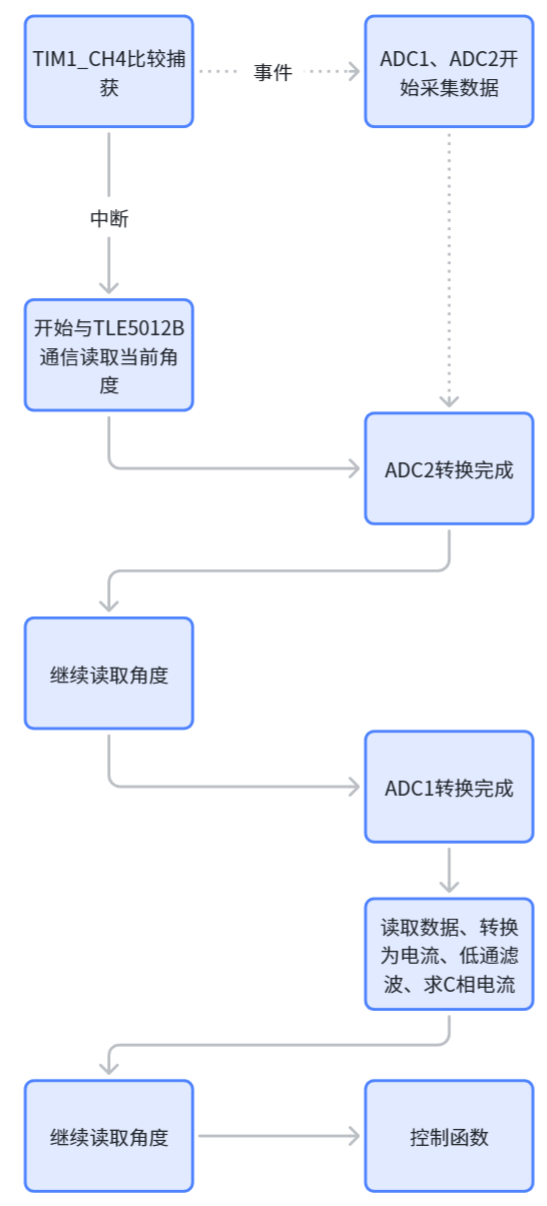
\includegraphics[width=0.2\textwidth]
    {图片/数据采集流程图.png}
    \caption{数据采集流程图}
    \label{fig:数据采集流程图}
\end{figure}

\begin{lstlisting}
    void HAL_ADCEx_InjectedConvCpltCallback(ADC_HandleTypeDef *hadc) {
    //ADC原始采样值
    extern uint32_t ADC_Data[3];
    //ADC转换后三相电流值
    extern float Current_abc[3];
    //ADC零位偏置
    extern float ADC1_ZERO;
    extern float ADC2_ZERO;
    //野值剔除暂存变量
    float Current_last[3];
    extern Discrete_PID_Struct Q_PID;
    //由于ADC1需要采集两个数据（其中有一个电压数据），ADC2只需要采集一个数据，因此ADC1总会比ADC2更晚进入中断
    if (hadc == &hadc1) {
        HAL_GPIO_WritePin(Test_GPIO_Port,Test_Pin, GPIO_PIN_SET);
        // ADC_Data[0] = HAL_ADCEx_InjectedGetValue(&hadc1, ADC_INJECTED_RANK_1);
        // ADC_Data[1] = HAL_ADCEx_InjectedGetValue(&hadc2, ADC_INJECTED_RANK_1);
        // ADC_Data[2] = HAL_ADCEx_InjectedGetValue(&hadc1, ADC_INJECTED_RANK_2);
        ADC_Data[0] = hadc1.Instance->JDR1;
        ADC_Data[1] = hadc2.Instance->JDR1;
        ADC_Data[2] = hadc1.Instance->JDR2;
        //野值剔除
        Current_last[0] = Current_abc[0];
        Current_last[1] = Current_abc[1];
        Current_last[2] = Current_abc[2];
        Current_abc[0] = -((ADC_Data[0] / 4096.0) * 3.3 - ADC1_ZERO) * 2;
        Current_abc[1] = -((ADC_Data[1] / 4096.0) * 3.3 - ADC2_ZERO) * 2;
        Current_abc[2] = -Current_abc[0] - Current_abc[1];
        if((Current_abc[0] > 0.45) || (Current_abc[0] < -0.45))
        {
            Current_abc[0] = Current_last[0];
            Current_abc[1] = Current_last[1];
            Current_abc[2] = Current_last[2];
        }
        else if((Current_abc[1] > 0.45) || (Current_abc[1] < -0.45))
        {
            Current_abc[0] = Current_last[0];
            Current_abc[1] = Current_last[1];
            Current_abc[2] = Current_last[2];
        }
        else if((Current_abc[2] > 0.45) || (Current_abc[2] < -0.45))
        {
            Current_abc[0] = Current_last[0];
            Current_abc[1] = Current_last[1];
            Current_abc[2] = Current_last[2];
        }
    }

    void HAL_TIM_PWM_PulseFinishedCallback(TIM_HandleTypeDef *htim) {
    if ((htim->Instance == TIM1) && (htim->Channel == HAL_TIM_ACTIVE_CHANNEL_4)) {
        //电流环运行标志位
        extern bool Current_Control_Flag;
        extern float theta;
        theta = TLE5012B_Angle();
        //如果电流环未运行，才进行电流环
        if (Current_Control_Flag == false)
        {
            Current_Control();
        }
    }
}
}
\end{lstlisting}

在控制函数中，主要执行计算电角度、进行克拉克-帕克变换求取当前的$I_d,I_q$、进行PID控制计算、SVPWM调制、设定三相占空比几个步骤。

克拉克-帕克变换需要相关的函数计算都已经用DSP库实现，只需要调用即可，相关函数如下所示。

\begin{lstlisting}
    void Clarke_Trans(float A, float B, float C, float *alpha, float *beta) {
        arm_clarke_f32(A, B, alpha, beta);
    }

   void Inv_Clarke_Trans(float alpha, float beta, float *A, float *B, float *C) {
        arm_inv_clarke_f32(alpha, beta, A, B);
        *C = 0 - *A - *B;   
    }

    void Park_Trans(float alpha, float beta, float Sin, float Cos, float *D, float *Q) {
        arm_park_f32(alpha, beta, D, Q, Sin, Cos);
    }

    void Inv_Park_Trans(float D, float Q, float Sin, float Cos, float *alpha, float *beta) {
        arm_inv_park_f32(D, Q, alpha, beta, Sin, Cos);
    }
\end{lstlisting}

采用PID控制器。在连续域中的传递函数为$G_{PID}(s)=K_p+\cfrac{K_i}{s}+K_d\cfrac{s}{\frac 1N s+1}$，采用双线性变换
$s=\cfrac{2}{T_s}\cfrac{1-z^{-1}}{1+z^{-1}}$，接下来推导采用双线性变换后的离散域传递函数与差分方程表示。

对于比例项保持不变为$K_p$，积分项双线性变换后为$\cfrac{K_iT_s}{2}\times\cfrac{1+z^{-1}}{1-z^{-1}}$

微分项的双线性变换后为$K_d\times\cfrac{2}{T_s}\cfrac{1-z^{-1}}{1+z^{-1}}\times\cfrac{1}{\frac{1}{N}\times
\frac{2}{T_s}\frac{1-z^{-1}}{1+z^{-1}}+1}$，
展开得到$\cfrac{2K_d}{T_s}\times\cfrac{NT_s(1-z^{-1})}{2(1-z^{-1})+NT_s(1+z^{-1})}$，化简可得
$\cfrac{2K_dN}{NT_s+2}\times\cfrac{1-z^{-1}}{1+\frac{NT_s-2}{NT_s+2}z^{-1}}$。

定义离散域下的系数$P=K_p,I=\cfrac{K_iT_s}{2},D=\cfrac{2K_dN}{NT_s+2},N_d=\cfrac{NT_s-2}{NT_s+2}$，则总的传递函数可以表示为
\begin{align*}
    G(z)&=P+I\cfrac{1+z^{-1}}{1-z^{-1}}+D\cfrac{1-z^{-1}}{1+N_dz^{-1}}\\
    & = \cfrac{P(1-z^{-1})(1+N_dz^{-1})+
    I(1+z^{-1})(1+N_dz^{-1})+
    D(1-z^{-1})^2}{(1-z^{-1})(1+N_dz^{-1})}\\
    & =\cfrac{(P+I+D)+(PN_d-P+IN_d+I-2D)z^{-1}+(D+IN_d-PN_d)z^{-2}}{1+(N_d-1)z^{-1}-N_dz^{-2}}\\
    & = \cfrac{Y(z)}{E(z)}
\end{align*}

由在控制系统中习惯采用增量式实现，增量式的传递函数为\(G'(z)=(1-z^{-1})G(z)\)，因此可得：
\begin{align*}
    G'(z)&=(1-z^{-1})G(z)\\
    & = \cfrac{(P+I+D)+(PN_d-2P+IN_d-3D)z^{-1}+(3D-2PN_d+P-I)z^{-2}+(PN_d-D-IN_d)z^{-3}}{1+(N_d-1)z^{-1}-N_dz^{-2}}\\
    & = \cfrac{b_0+b_1z^{-1}+b_2z^{-2}+b_3z^{-3}}{1+a_1z^{-1}+a_2z^{-2}}\\
    & = \cfrac{\Delta Y(z)}{E(z)}
\end{align*}

因此PID控制器结构体、初始化函数和执行的函数如下所示。

\begin{lstlisting}
    //PID控制器结构体
    typedef struct {
        float a1, a2;
        float b0, b1, b2, b3;
        float Error_Record[3];
        float Output_Delta_Record[2];
        float Error_Now;
        float Output_Delta_Now;
        float Setvalue;
    } Discrete_PID_Struct;

    //PID控制器结构体初始化函数
    void PID_Struct_Init(float Kp, float Ki, float Kd, float N, float Ts, float Default_Set, Discrete_PID_Struct* PID)
    {
        float P = Kp;
        float I = Ki * Ts / 2.0;
        float D = (2 * Kd * N) / (N * Ts + 2.0);
        float Nd = (N * Ts - 2.0) / (N * Ts + 2.0);
        if(Kd == 0)
        {
            Nd = 0;
            D = 0;
        }
        //增量式实现：输入误差，输出控制增量
        PID->Error_Record[0] = 0;
        PID->Error_Record[1] = 0;
        PID->Error_Record[2] = 0;
        PID->Output_Delta_Record[0] = 0;
        PID->Output_Delta_Record[1] = 0;
        PID->Error_Now = 0;
        PID->Output_Delta_Now = 0;
        PID->Setvalue = Default_Set;

        PID->a1 = -(Nd-1);
        PID->a2 = -(-Nd);
        PID->b0 = P + I + D;
        PID->b1 = P*Nd-2*P+I*Nd-3*D;
        PID->b2 = 3*D-2*P*Nd+P-I;
        PID->b3 = P*Nd-D-I*Nd;
    }

    //PID控制器执行函数
    void Discrete_PID_Controller(Discrete_PID_Struct* PID)
    {   
        //增量式实现：输入误差，输出控制增量
        float Temp_Output_Delta = 0;
        Temp_Output_Delta += PID->a1 * PID->Output_Delta_Record[0];
        Temp_Output_Delta += PID->a2 * PID->Output_Delta_Record[1];
        Temp_Output_Delta += PID->b0 * PID->Error_Now;
        Temp_Output_Delta += PID->b1 * PID->Error_Record[0];
        Temp_Output_Delta += PID->b2 * PID->Error_Record[1];
        Temp_Output_Delta += PID->b3 * PID->Error_Record[2];
        PID->Output_Delta_Now = Temp_Output_Delta;
        PID->Output_Delta_Record[1] = PID->Output_Delta_Record[0];
        PID->Output_Delta_Record[0] = PID->Output_Delta_Now;
        PID->Error_Record[2] = PID->Error_Record[1];
        PID->Error_Record[1] = PID->Error_Record[0];
        PID->Error_Record[0] = PID->Error_Now;
    }
\end{lstlisting}

SVPWM调制按照\eqref{eq:零序分量表达式}和\eqref{eq:SVPWM占空比表达式}计算即可。但根据电压极限圆表达式\eqref{eq:SVPWM电压极限圆}，
需要检查给定的$U_d,U_q$是否在电压极限圆内。如果不在电压极限圆内，需要进行线性放缩。相关函数如下所示。

\begin{lstlisting}
    void SVPWM_Calculation(float* Ud, float* Uq, float Sin, float Cos, float U_svpwm_max,float Udc,
    float* Duty_A, float* Duty_B,float* Duty_C)
    {
        float U_alpha, U_beta = 0;
        float U_ABC[3] = {0};
        float U_max, U_min = 0;
        float U_0 = 0;
        float u_mag = 0;
        if (U_svpwm_max == 0)
        {
            return;
        }
        arm_sqrt_f32((*Ud) * (*Ud) + (*Uq) * (*Uq), &u_mag);
        if (u_mag > U_svpwm_max)
        {
            u_mag = U_svpwm_max / u_mag;

        }
        else
        {
            u_mag = 1;
        }
        *Ud = (*Ud) * u_mag;
        *Uq = (*Uq) * u_mag;
        Inv_Park_Trans(*Ud, *Uq, Sin, Cos, &U_alpha, &U_beta);
        Inv_Clarke_Trans(U_alpha, U_beta, &U_ABC[0], &U_ABC[1], &U_ABC[2]);
        arm_max_f32(U_ABC, 3, &U_max, NULL);
        arm_min_f32(U_ABC, 3, &U_min, NULL);
        U_0 = -0.5 * (U_max + U_min);
        *Duty_A = 0.5 + (U_0 + U_ABC[0]) / Udc;
        *Duty_B = 0.5 + (U_0 + U_ABC[1]) / Udc;
        *Duty_C = 0.5 + (U_0 + U_ABC[2]) / Udc;
}   
\end{lstlisting}

为了增强程序的鲁棒性，避免后续在尝试更改PWM频率时需要连带修改程序，在设定三相占空比函数中通过用三相占空比乘ARR的值来确定需要给定的CCR。
相关函数如下所示。

\begin{lstlisting}
    void Set_CCR(float Duty_A, float Duty_B, float Duty_C) {
        int ARR = __HAL_TIM_GET_AUTORELOAD(&htim1);
        __HAL_TIM_SET_COMPARE(&htim1, TIM_CHANNEL_1, ARR*Duty_A);
        __HAL_TIM_SET_COMPARE(&htim1, TIM_CHANNEL_2, ARR*Duty_B);
        __HAL_TIM_SET_COMPARE(&htim1, TIM_CHANNEL_3, ARR*Duty_C);
    }   
\end{lstlisting}

最后调用上述函数的控制函数\texttt{void Current$\_$Control()}如下所示。

\begin{lstlisting}
    void Current_Control()
    {
        //机械角度
        extern float theta_m;
        extern float Angel_ZERO;
        //电角度
        extern float theta_e;
        //三相自然坐标系
        extern float Current_abc[3];
        //两相静止坐标
        extern float I_alpha;
        extern float I_beta;
        //同步旋转坐标系
        extern float I_d;
        extern float I_q;
        //三相占空比
        extern float Duty_A;
        extern float Duty_B;
        extern float Duty_C;
        //DQ轴电压
        extern float U_d;
        extern float U_q;
        //母线电压
        extern float Udc;
        //SVPWM最大电压
        extern float U_svpwm_max;
        //DQ轴电流控制器
        extern Discrete_PID_Struct D_PID;
        extern Discrete_PID_Struct Q_PID;
        //三角函数
        extern float Sin_theta_e;
        extern float Cos_theta_e;
        //电流环运行标志位
        extern bool Current_Control_Flag;
        //置位标志位
        Current_Control_Flag = true;
        //计算电角度
        theta_e = theta_m * MOTOR_POLE_PAIRS + Angel_ZERO;
        theta_e = fmod(theta_e, 360);
        theta_e<0?theta_e+=360:theta_e;
        //计算三角函数
        DSP_Float_Calc_SinCos(theta_e, &Sin_theta_e, &Cos_theta_e);
        //计算电流
        Clarke_Trans(Current_abc[0], Current_abc[1], Current_abc[2], &I_alpha, &I_beta);
        Park_Trans(I_alpha, I_beta, Sin_theta_e, Cos_theta_e, &I_d, &I_q);
        D_PID.Error_Now = D_PID.Setvalue - I_d;
        Q_PID.Error_Now = Q_PID.Setvalue - I_q;
        Discrete_PID_Controller(&D_PID);
        Discrete_PID_Controller(&Q_PID);
        U_d += D_PID.Output_Delta_Now;
        U_q += Q_PID.Output_Delta_Now;
        //SVPWM调制
        SVPWM_Calculation(&U_d, &U_q, Sin_theta_e, Cos_theta_e, U_svpwm_max, Udc, &Duty_A, &Duty_B, &Duty_C);
        // Q_PID.Output_Record[0] = U_q;
        // D_PID.Output_Record[0] = U_d;
        //设定CCR值
        Set_CCR(Duty_A, Duty_B, Duty_C);
        //重置标志位
        Current_Control_Flag = false;
        HAL_GPIO_WritePin(Test_GPIO_Port,Test_Pin, GPIO_PIN_RESET);
    }
\end{lstlisting}
由于采用了增量式的控制器实现形式，接收输入为每个控制周期中的偏差值，输出控制增量，天然具有很强的抗积分饱和特性，因此没有
使用额外的抗积分饱和手段。
通过给定$I_d$检测电流闭环控制效果。在给定$I_d=0.2A$和$I_d=-0.2A$情况下电流响应如下图所示。

\begin{figure}[H]
    \begin{minipage}{0.5\textwidth}
        \centering
        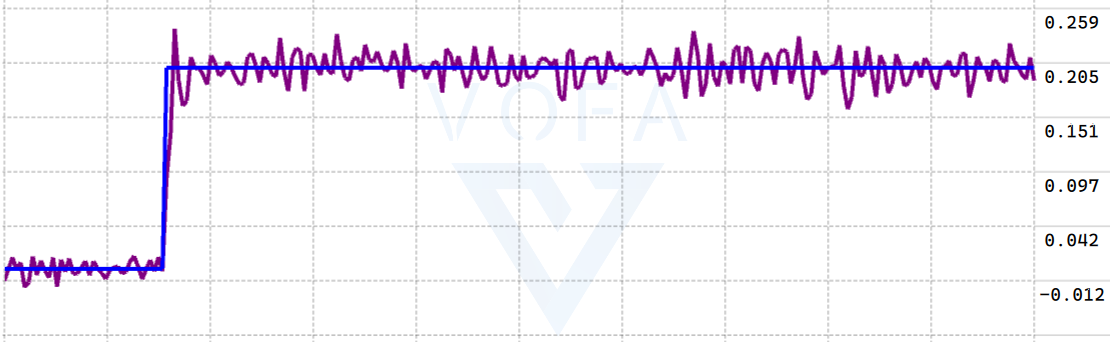
\includegraphics[width=1.1\textwidth]{图片/Id=0.2A阶跃响应图.png}
        \caption{$I_d$=0.2A阶跃响应图}
    \end{minipage}
    \begin{minipage}{0.5\textwidth}
        \centering
        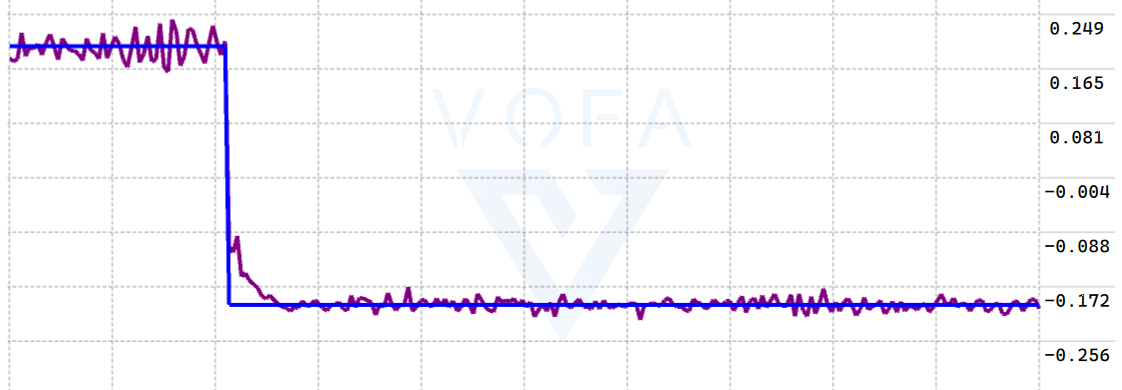
\includegraphics[width=1.1\textwidth]{图片/Id=-0.2A阶跃响应图.png}
        \caption{$I_d$=-0.2A阶跃响应图}
    \end{minipage}
\end{figure}

\subsection{速度外环PI闭环控制}

速度环的控制较之电流环基本一致，但是计算量上远不如电流环，控制周期也更长。因此选择向上位机传输数据的任务放在速度环控制周期中执行。

在TIM2的更新中断中进行数据采集，主要是求解此时的机械角速度（单位rpm），并且对母线电压采集结果转换为实际电压值，最后进入速度环控制函数。
相关函数如下所示。

\begin{lstlisting}
    void HAL_TIM_PeriodElapsedCallback(TIM_HandleTypeDef *htim) {
        extern float theta_m;
        extern float theta_m_last;
        extern float n_m;
        extern float n_m_last;
        extern float Udc;
        extern float U_svpwm_max;
        extern uint32_t ADC_Data[3];
        if (theta_m - theta_m_last < 10 && theta_m - theta_m_last > -10) {
            n_m = (theta_m - theta_m_last) / (Ts_Speed * 6);
        }
        n_m = (1-Speed_Filter) * n_m_last + Speed_Filter * n_m;
        n_m_last = n_m;
        theta_m_last = theta_m;
        Udc = ADC_Data[2] *0.00686;
        U_svpwm_max = Udc / SQRT3;
        Speed_Control();
        JUSTFLOAT_SendData();
    }
\end{lstlisting}

在速度环控制函数中，主要是执行速度环PID运算。采用$I_d=0$的控制策略，则速度环的输出就是Q轴电流环的给定值。为了避免堵转时速度环控制输出过高
导致Q轴电流环输出过高烧损电机，此处也需要对速度环控制器输出做限幅处理。相关函数如下所示。

\begin{lstlisting}
    void Speed_Control()
    {
        //DQ轴电流控制器
        extern Discrete_PID_Struct D_PID;
        extern Discrete_PID_Struct Q_PID;
        //速度环控制器
        extern Discrete_PID_Struct Speed_PID;
        //当前角速度
        extern float n_m;
        //速度环给定限幅
        if(Speed_PID.Setvalue < -Speed_Target_Limit)
        {
            Speed_PID.Setvalue = -Speed_Target_Limit;
        }
        else if(Speed_PID.Setvalue > Speed_Target_Limit)
        {
            Speed_PID.Setvalue = Speed_Target_Limit;
        }
        Speed_PID.Error_Now = Speed_PID.Setvalue - n_m;
        Discrete_PID_Controller(&Speed_PID);
        Q_PID.Setvalue += Speed_PID.Output_Delta_Now;
        //采用Id=0，Iq给定的控制策略
        if (Q_PID.Setvalue < -Speed_Output_Limit)
        {
            Q_PID.Setvalue = -Speed_Output_Limit;
        }
        else if (Q_PID.Setvalue > Speed_Output_Limit)
        {
            Q_PID.Setvalue = Speed_Output_Limit;
        }
    }
\end{lstlisting}
采用给定速度值300rpm，速度环输出限幅0.5A。无负载情况下的速度阶跃响应如下图所示（纵轴单位rpm）。
\begin{figure}[H]
    \centering
    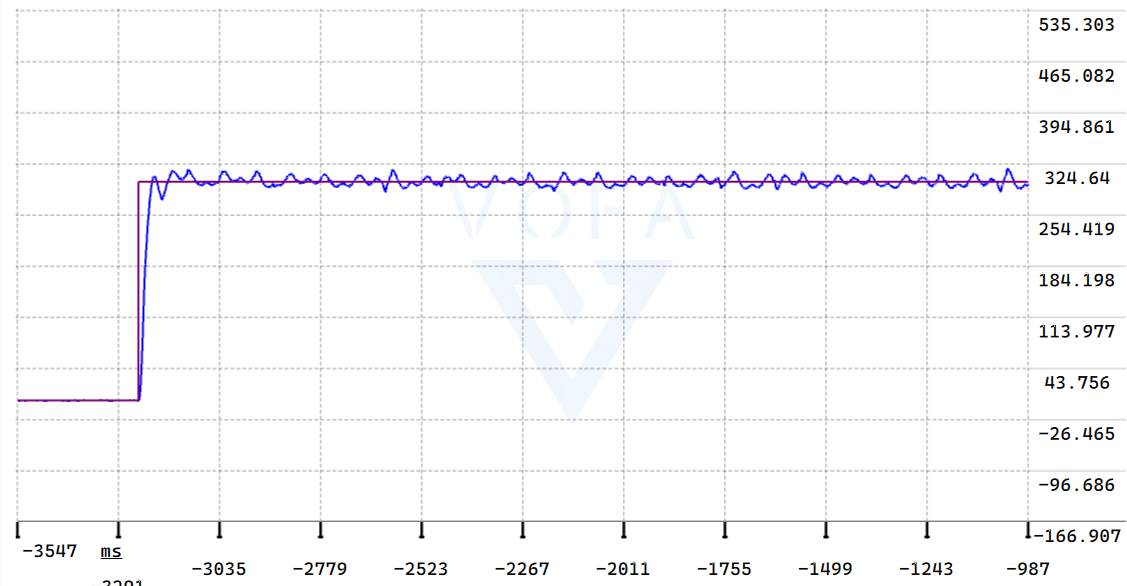
\includegraphics[width=0.6\textwidth]
    {图片/速度阶跃响应图.png}
    \caption{$n_m=300rpm$阶跃响应图}
\end{figure}

通过设置速度环输出限幅，能够确保在堵转情况下电机的安全性。在上述条件下堵转电机，DQ轴电流响应如下图所示（紫线表示
$I_d$，粉线表示$I_q$）。
\begin{figure}[H]
    \centering
    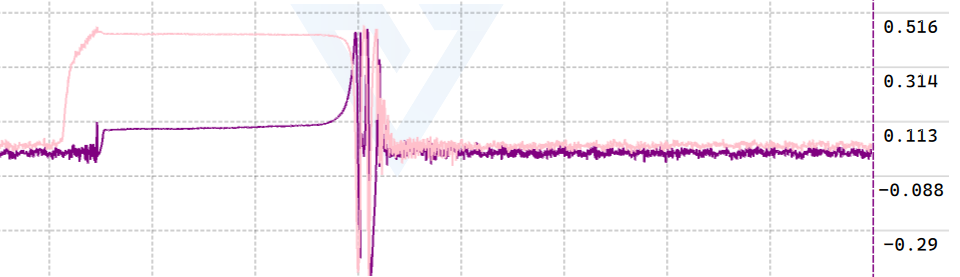
\includegraphics[width=0.6\textwidth]
    {图片/DQ电流响应图.png}
    \caption{DQ轴电流响应图}
\end{figure}

上述过程中，当堵转发生时，反电动势消失，导致DQ电流同时升高，直到控制输出电压达到SVPWM调制极限。松开时，
由于增量式控制器对饱和的天然抵抗性，能够快速的实现退饱和。

另外，为了方便调试，通过UART4的DMA接收不定长数据的功能，通过接收上位机传来的指令来调整设定值，其中断回调函数如下所示。
\begin{lstlisting}
    void HAL_UARTEx_RxEventCallback(UART_HandleTypeDef *huart, uint16_t Size) {
    extern uint8_t  UART_Buffer[100];
    extern float Order;
    extern uint16_t UART_Length;
    extern Discrete_PID_Struct D_PID,Q_PID,Speed_PID;
    UART_Length = Size;
    if (UART_Length > 0 && UART_Length < 100)
    {
        UART_Buffer[UART_Length] = '\0';
        Order = atof((const char *)UART_Buffer);
    }
    HAL_UARTEx_ReceiveToIdle_DMA(&huart4, UART_Buffer, 100);
    //以下三个选择其一进行设置
    Speed_PID.Setvalue = Order;
    // D_PID.Setvalue = Order;
    // Q_PID.Setvalue = Order;
}
\end{lstlisting}